% Chapter 5

\chapter{Results} % Main chapter title
\label{chapter:results} % For referencing the chapter elsewhere, use \ref{Chapter1} 
This chapter presents the findings from the methodologies employed throughout this study.
The focus of the research was to identify the material parameters of ultra-soft polyurethane
effectively. The results obtained offered critical insights into the approach's 
efficacy and potential limitations.\\

In the first section, the performance metrics applied were examined. These metrics 
provided a quantifiable measure of the validity and reliability of the material parameter sets identified,
offering a robust means of assessing the approach's accuracy.

Subsequently, a thorough analysis of the three validation cases are detailed.
These cases contributed significantly to select the best material parameter set and 
assess the applicability of the material parameters in other use cases.

This is followed by a detailed exposition of the framework proposed in this study for the material 
parameter identification process based on an iFEM approach.

Lastly, the limitations and implications of the results are listed. By identifying the constraints 
of the results, a well-rounded perspective of the findings was presented to further refine the 
process for future research.

%----------------------------------------------------------------------------------
\section{Overview and Analysis}
Upon applying the RSO and MATLAB optimization to identify the optimal material parameter set, 
multiple sets were calculated. 
Each simulation deployed various Neo-Hookean parameters sets and 
had a unique load-displacement solutions. These load-displacement curves were 
juxtaposed with the experimental data and the RMSE and NRMSE (Equation \ref{eq:rmse} and \ref{eq:nrmse}) was calculated to quantify the quality 
of each solution. To deepen the evaluation, additional performance metrics were incorporated: 
Mean Relative Error (MRE) (Equation \ref{eq:mre}), Mean Absolute Percentage Error (MAPE)
\begin{align}
    \text{MAPE} = \frac{100\%}{n} \sum_{i=1}^{n} \left| \frac{y_i - \hat{y}_i}{y_i} \right| \,,
\end{align}
and  Relative Root Mean Square Error (RRMSE)  
\begin{align}
    \text{RRMSE} = \sqrt{\frac{1}{n} \sum_{i=1}^{n} \left( \frac{y_i - \hat{y}_i}{y_i} \right)^2} \,.
\end{align}
%https://www.analyticsvidhya.com/blog/2021/10/evaluation-metric-for-regression-models/   
Performance metrics are critical for evaluating the predictive accuracy of the computational model.
These metrics provide insights into how well the model's prediction align with the 
experimental data. The combination of these metrics allowed for a more comprehensive 
assessment of all the simulations performance. For instance, the RMSE and NRMSE measured the
absolute deviation of the predicted values from the observed data, providing an overall 
measure of the computational model accuracy. On the other hand, metrics like MRE, MAPE. and 
RRMSE are useful when considering relative errors. These metrics weighed errors in relation
to the actual size of the actual values \cite{Rajagukguk2020}.\\

The simulation results that produced the lowest performance metrics were set aside as possible
optimal candidates. In particular, the parameters with the lowest NRMSE, MRE and RMSRE were  
investigated. Moreover, a set with an elevated incompressibility parameter was chosen for 
analyzing its influence on validation cases.
The parameters that were determined to provide the best fit to the 
experimental data based on these assessments were listed on Table \ref{tab:materialsetbestfit}.
\begin{table}[ht!]
    \centering
    \begin{tabular}{|c|c|c|c|c|c|c|}
    \hline
    Set & $\mu$ (Pa) & $D_1$ (MPa\textsuperscript{-1}) & NRMSE & MRE & RRMSE & Optimization Method\\
    \hline
    1 & 9999.7 & 5.8 & \textbf{0.0339} & 0.1098 & 0.2067 & RSO 2P RR\\
    2 & 9975.2 & 5.3 & 0.0340 & \textbf{0.1097} & 0.2069 & RSO 2P RR\\
    3 & 10200 & 1.1 & 0.0533 & 0.1139 & \textbf{0.1964} & MATLAB Poly 4 MRE\\
    4 & 12453 & 139.3 & 0.0648 & 0.1713 & 0.2592 & RSO 2P FR\\
    \hline
    \end{tabular}
    \caption[Best material parameter sets]{Neo-Hookean material parameter sets that demonstrated the best fit to the experimental data of the EM II.}
	\label{tab:materialsetbestfit}
\end{table}

\subsection*{Assessment of Performance Metrics}
Defining good performance metrics values required a multi-dimensional approach. 
Firstly, the load-displacement curves' visual inspection revealed a close approximation 
to the experimental data (Fig. \ref{fig:bestfitcandidatescurve}).

The load-displacements curves illustrated that the initial slope of EM II was steeper compared to 
all calculated candidate sets. As the displacement increased sets \SI{1}{} through \SI{3}{} intersected 
the experimental curve. Set \SI{1}{} and \SI{2}{} were nearly identical, initially exhibited an increasing 
slope, yet displayed a tendency to flatten towards the end of the curve, intersecting the experimental curve 
a second time.

On the other hand, set \SI{3}{} crossed the experimental curve around $u=\SI{1.5}{\milli \meter}$, showcasing 
a steeper slope relative to the experimental curve. 

Set \SI{4}{} displayed a pronounced curvature at the outset, followed by an increase in steepness of its slope.
However, it remained constantly below throughout the experimental data.\\

%load-displacements results curves comparison
\begin{figure}%
    \centering
   \quad
    \begin{tikzpicture}[scale=1]
        \begin{axis}[
            xmax=4.2,xmin=0,
            ymin= 0,ymax=0.6,
            ytick={0,0.1,0.2,...,0.5},
            xlabel={Displacement $u [mm]$},
            ylabel={Force reaction $F_{II} [N]$},
            grid = major,
            legend pos= north west]
            \addplot+[smooth, no markers, thick] table [y=$Force$, x=Def]{Table/RSO/expdatatop.dat};
            \addplot+[smooth, no markers, thick] table [y=$Force$, x=Def]{Table/results/set199997_58.dat};
			\addplot+[smooth, no markers, thick] table [y=$Force$, x=Def]{Table/results/set299752_53.dat};
            \addplot+[smooth, no markers, thick] table [y=$Force$, x=Def]{Table/results/set310200_11.dat};
            \addplot+[smooth, orange, no markers, thick] table [y=$Force$, x=Def]{Table/results/set412453_1393.dat};
            \legend{EM II-MP,Set 1,Set 2, Set 3, Set 4}
        \end{axis}
    \end{tikzpicture}%
   \caption[Best material parameter sets load-displacement curves]{Visual analysis of the load-displacement curves of the best material parameter sets with the lowest NRMSE, MRE, and RRMSE and the experimental data.}%
   \label{fig:bestfitcandidatescurve}%
\end{figure}

In addition to the visual analysis, the mean of the performance metrics for all models were calculated and 
compared to its lowest value. Similarly, a baseline model of each performance metric was calculated and 
also compared to the candidate sets (Table \ref{tab:performancegoodness}). 

To clarify, the lowest value of the NRMSE was $\SI{0.0339}{}$. The mean NRMSE across all models was 
$\SI{0.1662}{}$, suggesting that models with an NRMSE below this value outperformed the average.
Consequently, the baseline NRMSE, represented a simple model predicting the mean load-displacement, was 
$\SI{0.6835}{}$, indicating that models with an NRMSE below this value surpassed the baseline model.\\ 

\begin{table}[ht!]
    \centering
    \begin{tabular}{|>{\centering\arraybackslash}m{2cm}|>{\centering\arraybackslash}m{2cm}|>{\centering\arraybackslash}m{2cm}|>{\centering\arraybackslash}m{2cm}|}
    \hline
    Metric & Set values & Mean & Baseline \\
    \hline
    NRMSE &  0.0339 0.0340 0.0533 0.0648 & 0.1662 & 0.6835 \\
    \hline
    MRE &  0.1098 0.1097 0.1139 0.1713 & 0.2689 & 0.5916\\
    \hline
    RRMSE & 0.2067 0.2069 0.1964 0.2592 & 0.2688 & 0.6835\\
    \hline
    \end{tabular}
    \caption[Goodness of fit]{Comparison of the performance metric of each candidate set with their mean value and baseline model value, extracted from all calculated simulations.}
	\label{tab:performancegoodness}
\end{table}

Given the proximity of the values among all candidates, except for set \SI{4}{}, it was 
initially inferred that utilizing NRMSE as the sole performance metric would be adequate for 
evaluating the goodness of fit in this specific case, an indentation of $h=\SI{4}{\milli \meter}$
at the center of the surface.

\section{Validation of Computational Model}
\label{section:validationcm}
In order to confirm the reliability and effectiveness of the identified material parameters,
two distinct validation cases were performed. 
The first validation case (VC I) involved the alteration of the indentation depth, changing it to 
$\SI{8}{\milli \meter}$ from the original $\SI{4}{\milli \meter}$. This case aimed to assess how 
well the material model could adapt and represent the mechanical behavior with increased deformation.

The second validation case (VC II)  revolved around the deformation profile of the spe-\\cimen. The aim here 
was understand the accuracy in predicting the actual deformation shape of the specimen under 
indentation. This provided deeper insights into the effects of the selected incompressibility
parameters.\\

The experimental models for the validation cases followed the same procedural guidelines 
described in Chapter \ref{chapter:experimentalmodel} for experimental model II. 
Furthermore, for the validation cases only Sets \SI{1}{}, \SI{3}{} and \SI{4}{} were evaluated (Table \ref{tab:materialsetbestfit}).
As set \SI{2}{} demonstrated nearly identical results as set \SI{1}{}, it was not considered for the 
validation process.

\subsection{Deeper Indentation}
\label{subsection:8mm}
The first validation experiment featured an indentation depth of $h_{VC1}=\SI{8}{\milli \meter}$,
doubling the previous indentation depth of $h=\SI{4}{\milli \meter}$ at the center of the specimen's 
surface or middle point. Computational model II, described in Chapter \ref{chapter:computationalmodel},
was used with the adjusted indentation depth (Fig. \ref{fig:stressdis8mm}).\\

\begin{figure}%
	\centering
   \quad
   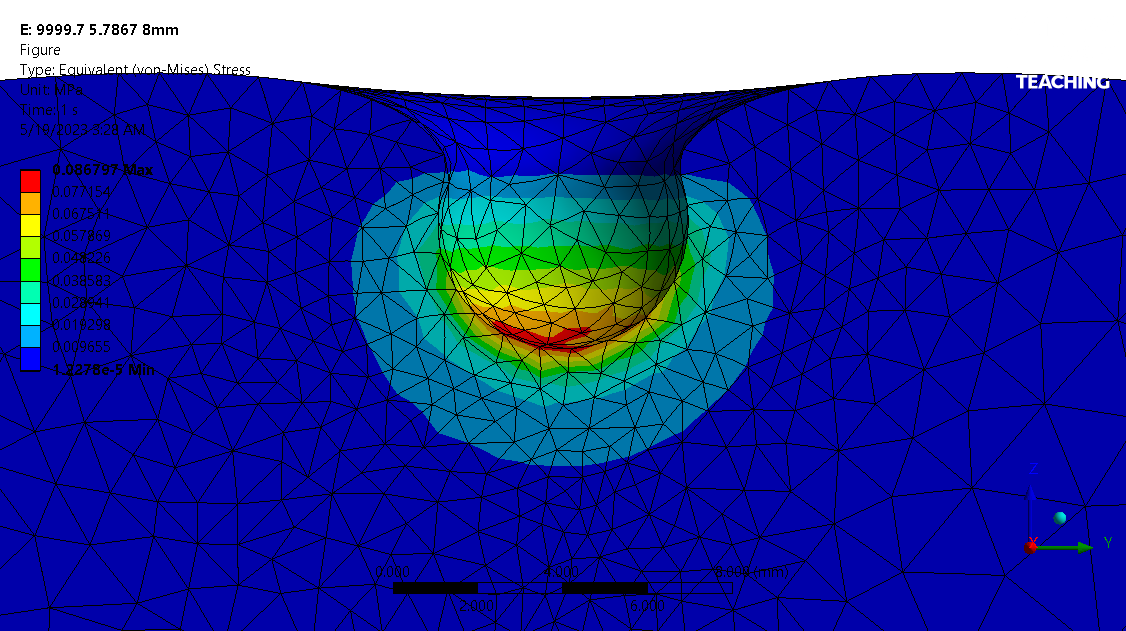
\includegraphics[width=10cm]{Images/validationcase/8mm/setstressdistribution.png}%
   \caption[Deeper Indentation - Stress distribution]{Stress distribution and meshing for the first validation case with an indentation depth of $h_{VC1}=\SI{8}{\milli \meter}$.}%
   \label{fig:stressdis8mm}%
\end{figure}
%Here stress distribution description

To facilitate the comparison of the remaining candidates, the load-displacement curves for the 
set \SI{1}{} with the lowest NRMSE, set \SI{3}{} with the lowest RRMSE, and set \SI{4}{}  with the highest 
incompressibility parameter, were plotted against the experimental data, as shown in Figure \ref{fig:8mmloaddisplcurves}.\\ 
%8mm load displacement curves
\begin{figure}%
    \centering
   \quad
    \begin{tikzpicture}[scale=1]
        \begin{axis}[
            xmax=8.5,xmin=0,
            ymin= 0,ymax=1.5,
            ytick={0,0.2,...,1.4},
            xlabel={Displacement $u [mm]$},
            ylabel={Force reaction $F_{II} [N]$},
            grid = major,
            legend pos= north west]
            \addplot+[smooth, no markers, thick] table [y=$Force$, x=Def]{Table/results/8mm/expdatatop8mm.dat};
            \addplot+[smooth, no markers, thick] table [y=$Force$, x=Def]{Table/results/8mm/set199997_58_8mm.dat};
            \addplot+[smooth, no markers, thick] table [y=$Force$, x=Def]{Table/results/8mm/set310200_11_8mm.dat};
            \addplot+[smooth, no markers, thick] table [y=$Force$, x=Def]{Table/results/8mm/set412453_1393_8mm.dat};
            \legend{EM II-VC I, Set 1, Set 3, Set 4}
        \end{axis}
    \end{tikzpicture}%
   \caption[First validation case load-displacement curves]{Analysis of the load-displacement curves of the best material parameter sets and the experimental data for the first validation case with a deeper indentation.}%
   \label{fig:8mmloaddisplcurves}%
\end{figure}

The load-displacement graph showed that the experimental data displayed again a steeper initial slope 
than the computational models. Sets \SI{1}{} and \SI{3}{} curves intersected the experimental curve 
around a displacement of $u=\SI{2}{\milli \meter}$, whereas set \SI{4}{} intersected at about $u=\SI{3}{\milli \meter}$.

As displacement increased to $u=\SI{4}{\milli \meter}$, the curves for sets \SI{1}{} and \SI{3}{} began 
to flatten and fell beneath the experimental curve, while set \SI{4}{} maintained its steepness and remained above.
At a displacement of $u=\SI{8}{\milli \meter}$, set \SI{4}{} with a maximum force of 
$F_{4_{max}}=\SI{1.3951}{\newton}$ managed to produce the closest 
approximation to the maximum experimental force $F_{II_{max}}=\SI{1.283}{\newton}$.

The new NRMSE values were significantly higher than those of the first case (Table \ref{tab:nrmse8mm}). 
Noteworthy, set \SI{3}{}, with a lower NRMSE for the first case, and set \SI{4}{} with a higher $D_1$ 
exhibited a better NRMSE performance for this case, in contrast to set \SI{1}{}, which had shown 
the best performance for the $h=\SI{4}{\milli \meter}$ indentation.\\

\begin{table}[ht!]
    \centering
    \begin{tabular}{|c|c|c|c|c|}
    \hline
    Set & $\mu$ (Pa) & $D_1$ (MPa\textsuperscript{-1}) & EM II NRMSE & VC I NRMSE\\
    \hline
    1 & 9999.7 & 5.8 & 0.0339 & 0.1503\\
    \textbf{3} & \textbf{10200} & \textbf{1.1} & 0.0533 & \textbf{0.1116}\\
    4 & 12453 & 139.3 & 0.0648 & 0.1425\\
    \hline
    \end{tabular}
    \caption[NRMSE for first validation case]{Comparison of the NRMSE calculated for the EM II and for the first validation case with a deeper indentation.}
	\label{tab:nrmse8mm}
\end{table}

This suggested that the identified parameters may not be able to capture the behavior 
of the material at larger indentations. Therefore, a case-specific parameter identification
for accurate modelling of larger indentations would be required.\\

%------------------------------------------------------------------------------------------------
\subsection{Deformation Profile Analysis}
\label{subsection:defprofanalysis}
The second validation case evaluated the deformation profile of the specimen for the first 
indentation case of $h=\SI{4}{\milli \meter}$ in the middle of the specimen's surface. The goal 
was to understand how the selection of the incompressibility parameter, linked to the 
bulk modulus, influenced the deformation shape under indentation.\\

To capture the deformation shape of the specimen, the displacement of the points along an axis positioned 
$\SI{5}{\milli \meter}$ parallel to the X-axis were calculated (Fig. \ref{fig:defprofdiagram}). %Figure of diagram of
This reference line was chosen to avoid any optical interference caused by the indenter during the 
laser measurements, as illustrated in Figure \ref{fig:defprofinter}.
Figure \ref{fig:defprofexperiment} illustrates the experiment conducted by YNU.
Using the marked points as reference, the laser displacement meter captured the specimen's 
shape along the parallel axis both before and during the indentation process.
This allowed for the measurement of the deformation profile at intervals of $\SI{1}{\milli \meter}$
throughout the indentation until reaching the maximum depth of $\SI{4}{\milli \meter}$ was reached (Appendix \ref{AppendixA}).\\

\begin{figure}%
	\centering
   \quad
   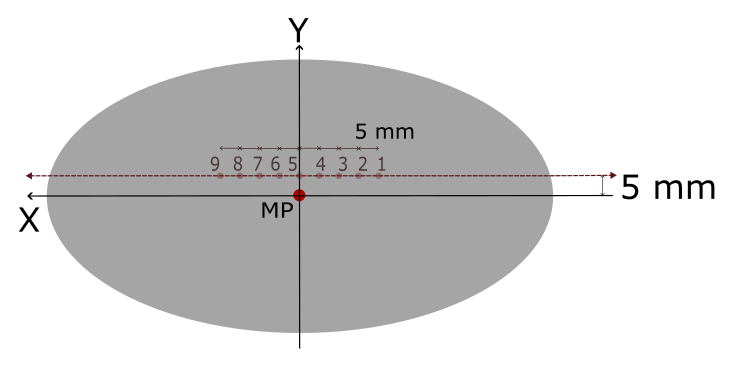
\includegraphics[width=10cm]{Images/validationcase/defprof/defprofdiag.png}%
   \caption[Deformation profile - Diagram]{Deformation profile measurement diagram for the second validation case, showing the measured points along the parallel to X-axis.}%
   \label{fig:defprofdiagram}%
\end{figure}

\begin{figure}
    \centering
    \begin{subfigure}[b]{0.5\textwidth}
    \centering
    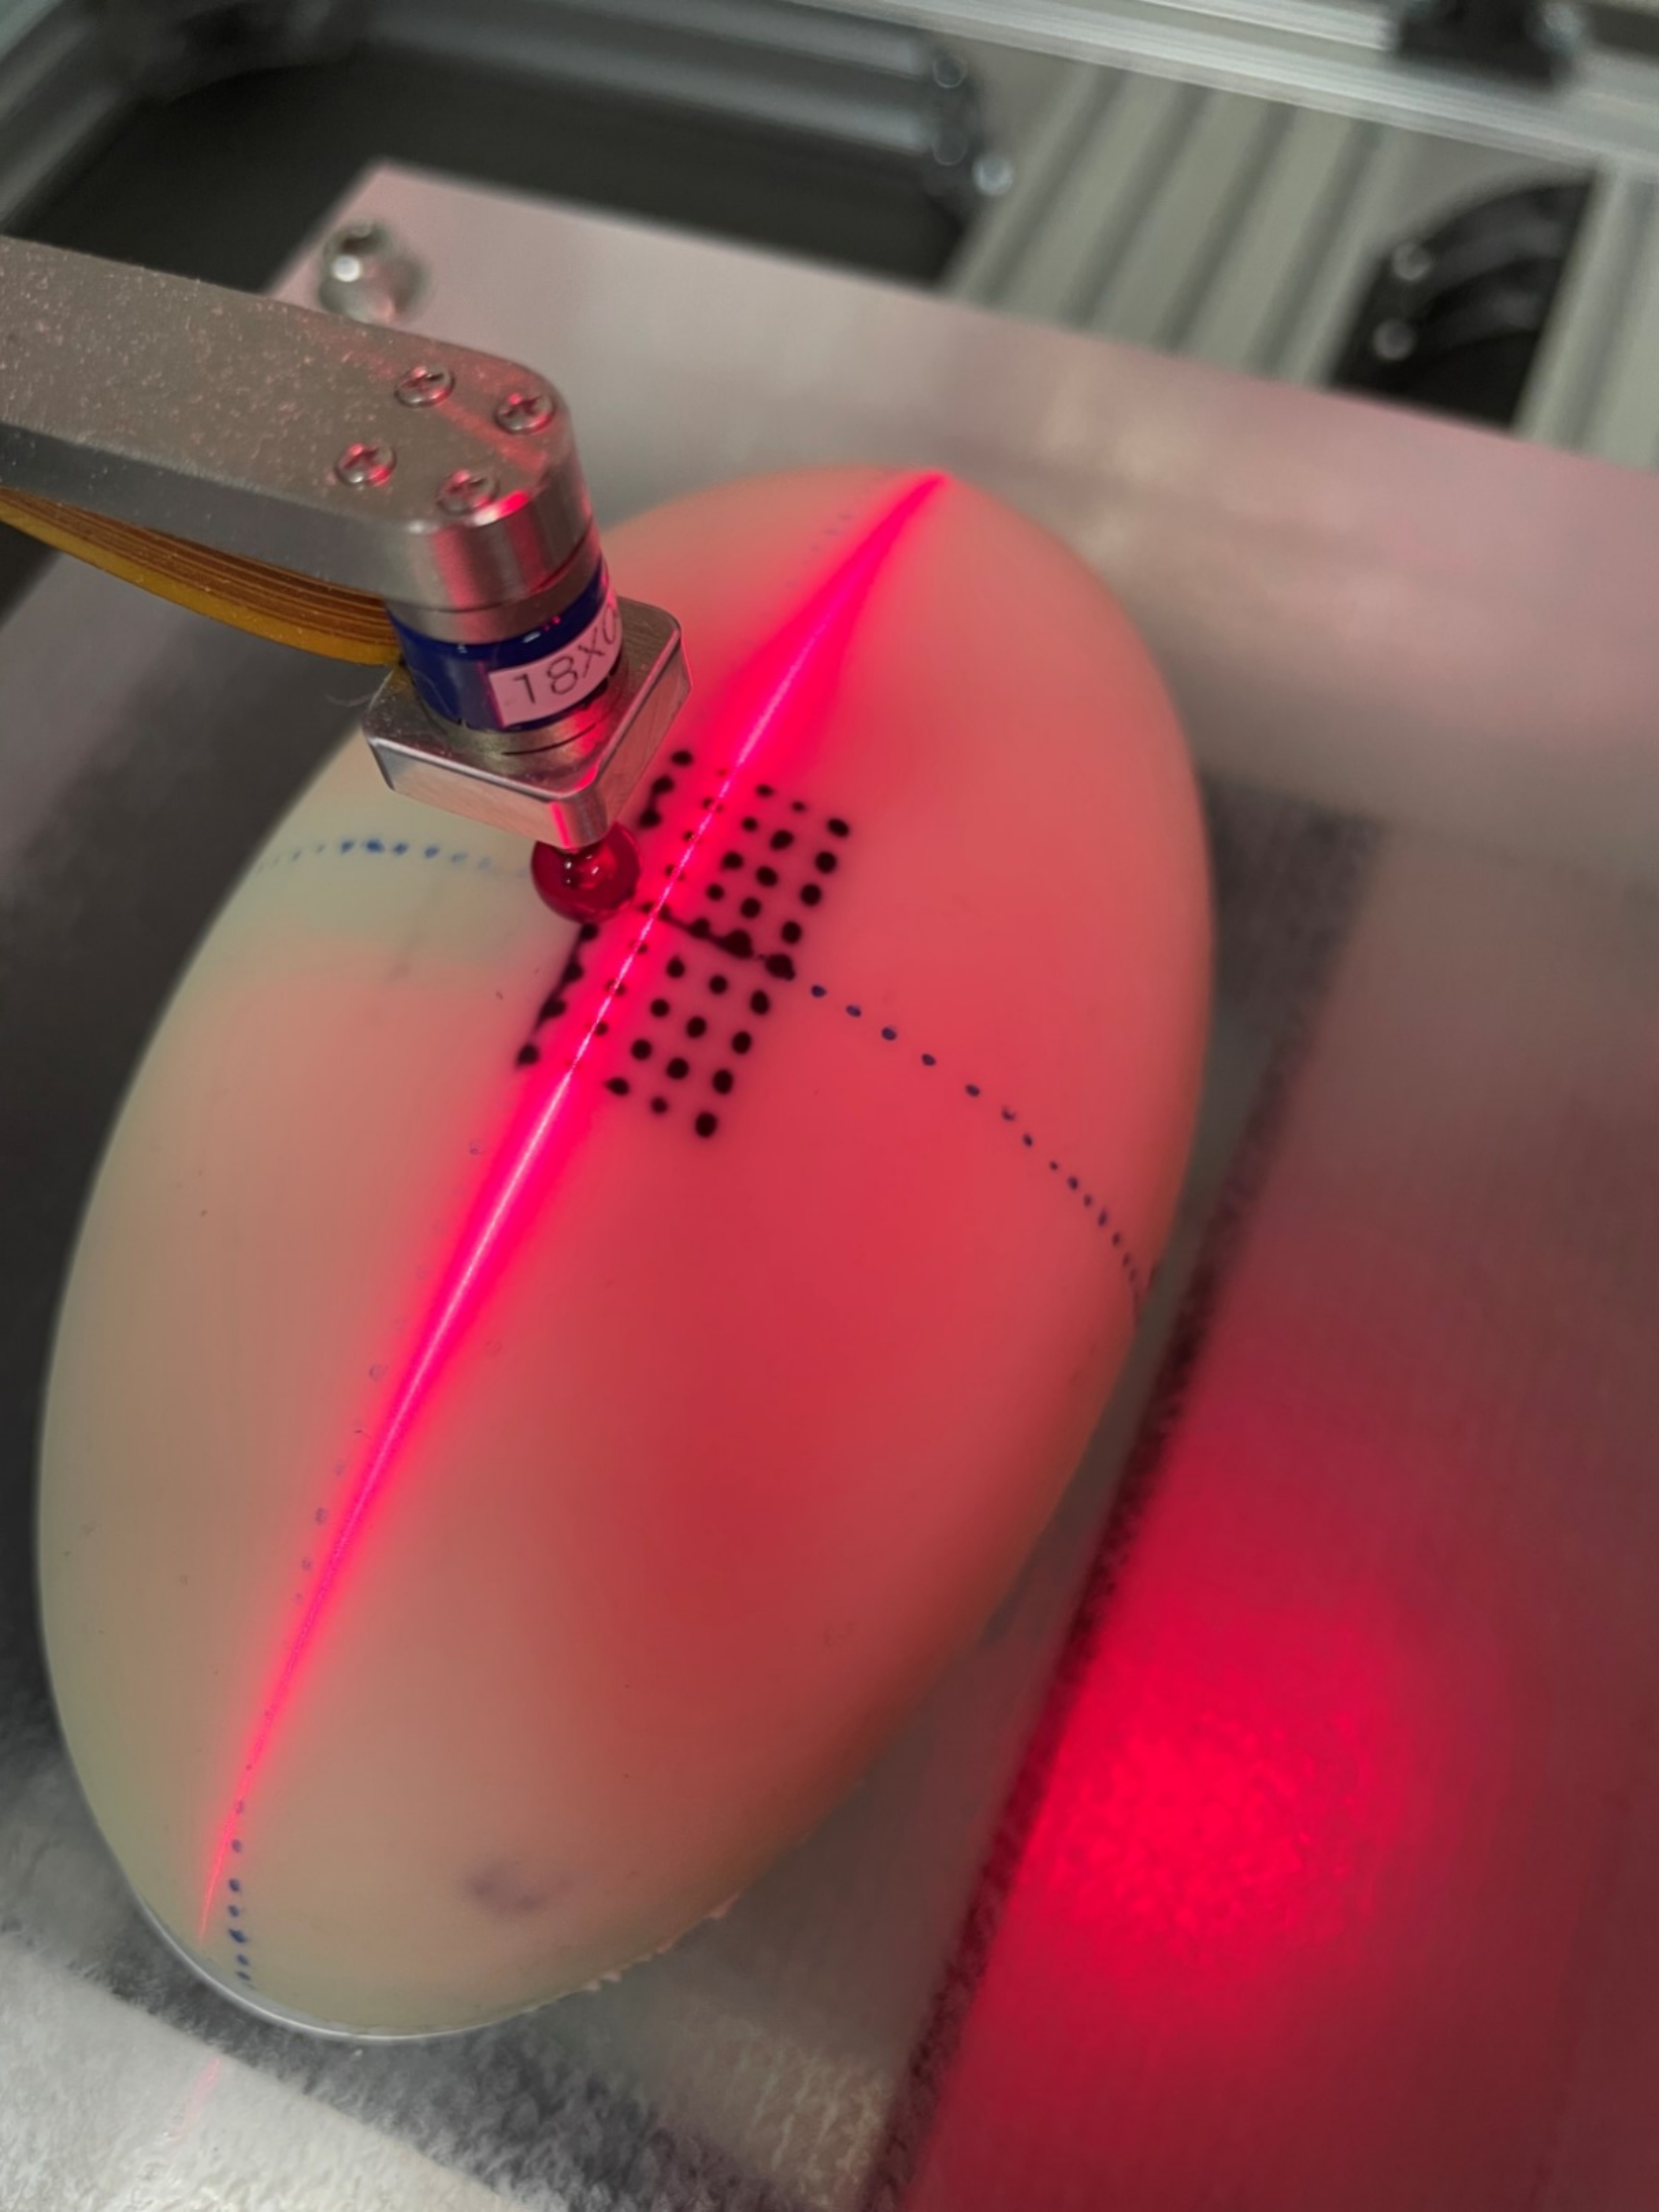
\includegraphics[width=\textwidth]{Images/validationcase/defprof/defprofexp.png}
    \caption{Experimental setup with laser displacement meter measurement}
    \label{fig:defprofexce}
    \end{subfigure}
    \hfill
    \begin{subfigure}[b]{0.5\textwidth}
    \centering
    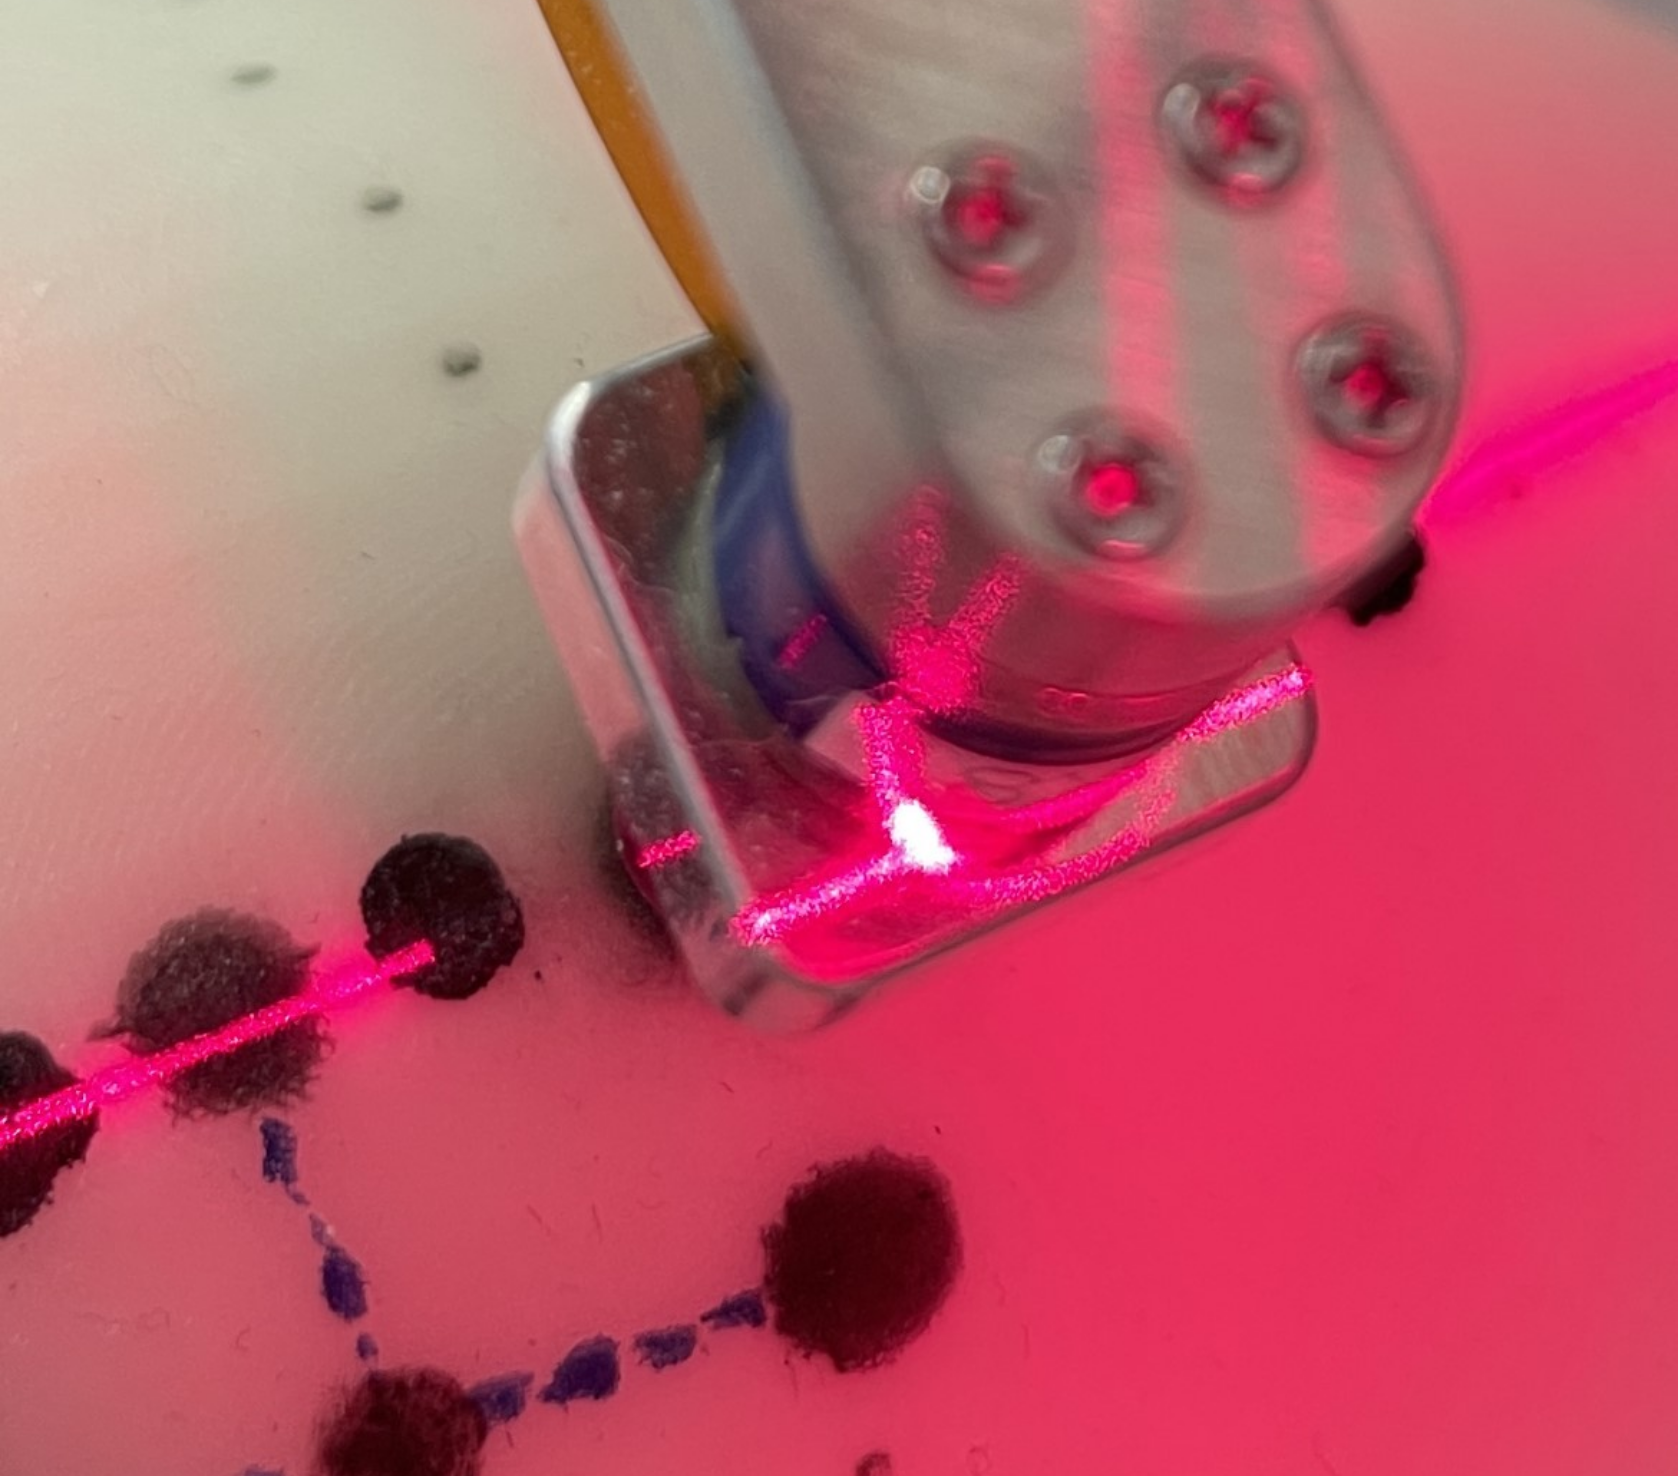
\includegraphics[width=\textwidth]{Images/validationcase/defprof/interferencedef.png}
    \caption{Interference from the indenter of the measurements along the main X-axis}
    \label{fig:defprofinter}
    \end{subfigure}
    \hspace{0.3cm}
    \caption[Deformation profile experiment]{Deformation profile experiment setup performed by YNU to capture the shape of the specimen during the indentation test.}
    \label{fig:defprofexperiment}
\end{figure}

From the results calculated with the computational model II for the middle point case, 
a method to capture the deformation profile for the second validation case was required.
However, tracking specific points on the surface of the simulation was challenging due to 
the remeshing process of the nonlinear adaptive meshing option utilized in the model. This
process did not support the measurement of the displacement for a specific node, as the 
position of the node changed throughout the execution of the model's calculation.\\

To overcome this issue, a section plane was created, located $\SI{5}{\milli \meter}$ to the 
right of the symmetry axis, similar to the experimental model. Probe points were then
selected around the deformed surface within this plane (Fig. \ref{fig:defprofcompmodel}).

\begin{figure}%
	\centering
   \quad
   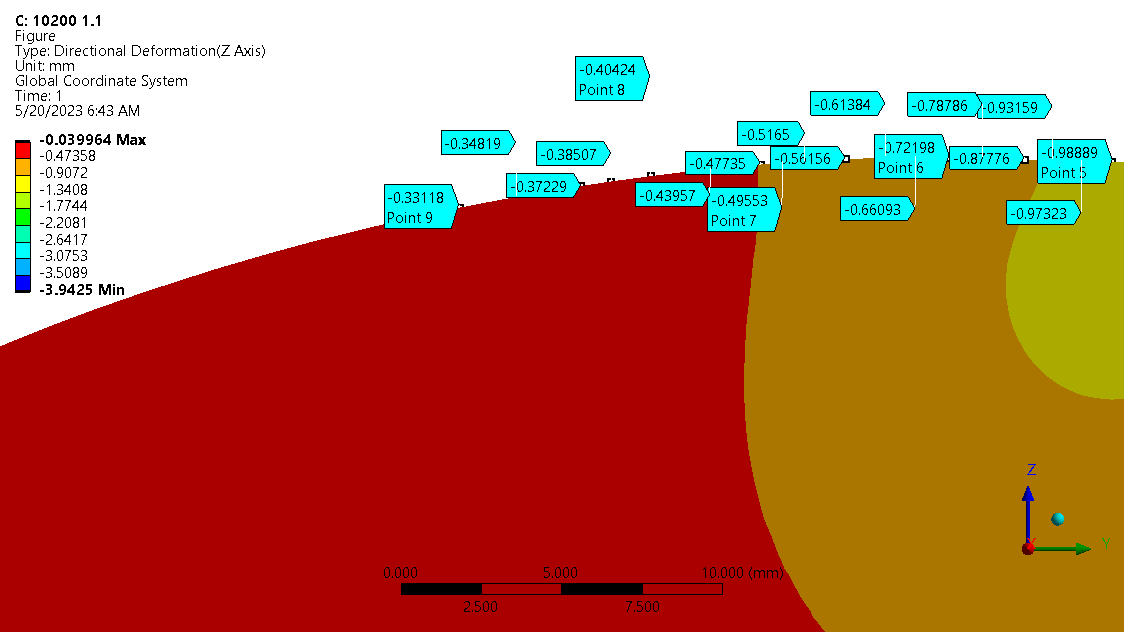
\includegraphics[width=10cm]{Images/validationcase/defprof/10200defprofile.png}%
   \caption[Deformation profile - Computational model]{Deformation profile measurement in the computational model with aid of probes along the surface of the section plane located $\SI{5}{\milli \meter}$ next to the X-axis.}%
   \label{fig:defprofcompmodel}%
\end{figure}

The deformation profiles for the remaining candidate sets were compared with the experimental
data, as shown in Figure \ref{fig:defprofiledata}. Although all computational models 
showed some degree of misalignment with the experimental data, the position of maximum deformation,
Point \SI{5}{} next to middle point, had a close match for sets \SI{1}{} and \SI{3}{}.

Further, as the incompressibility parameter decreased, the overall deformation decreased. The 
NRMSE values for this case were listed on Table \ref{tab:nrmsedefprof}. The NRMSE results 
revealed that the set \SI{3}{} had the best value followed closely by set \SI{1}{}. This validation case 
showcased that the selection of the range set for the iFEM process impacts the deformation response, even though the
influence of the incompressibility parameter on the force reaction results was relatively minor.\\
\begin{table}[ht!]
    \centering
    \begin{tabular}{|c|c|c|c|c|}
    \hline
    Set & $\mu$ (Pa) & $D_1$ (MPa\textsuperscript{-1}) & EM II NRMSE & VC II NRMSE\\
    \hline
    1 & 9999.7 & 5.8 & 0.0339 & 0.3126\\
    \textbf{3} & \textbf{10200} & \textbf{1.1} & 0.0533 & \textbf{0.2810}\\
    4 & 12453 & 139.3 & 0.0648 & 0.5645\\
    \hline
    \end{tabular}
    \caption[NRMSE for second validation case]{Comparison of the NRMSE calculated for the EM II and for the second validation case for the deformation profile curves.}
	\label{tab:nrmsedefprof}
\end{table}

\begin{figure}%
    \centering
   \quad
    \begin{tikzpicture}[scale=1]
        \begin{axis}[
            xmax=25,xmin=0,
            ymax= 0,ymin=-1.4,
            ytick={0,-0.2,...,-1.4},
            xlabel={X-Axis displacement $u_{x} [mm]$},
            ylabel={Z-Axis displacement $u_{x} [mm]$},
            grid = major,
            legend pos= south east]
            \addplot+[smooth, thick] table [y=$Def$, x=Xdis]{Table/results/defprofile/defprofexp.dat};
            \addplot+[smooth, no markers, thick] table [y=$Def$, x=Xdis]{Table/results/defprofile/set1prof.dat};
            \addplot+[smooth, no markers, thick] table [y=$Def$, x=Xdis]{Table/results/defprofile/set3prof.dat};
            \addplot+[smooth, no markers, thick] table [y=$Def$, x=Xdis]{Table/results/defprofile/set4prof.dat};
            \legend{EM II-VC II, Set 1, Set 3, Set 4}
        \end{axis}
    \end{tikzpicture}%
   \caption[Second validation case measurement data]{Analysis of the deformation profile curves of the best material parameter sets and the experimental data for the second validation case.}%
   \label{fig:defprofiledata}%
\end{figure}

Based on the combined results of both validation cases and their NRMSE values, set 3 with a 
shear modulus $\mu=\SI{10200}{\pascal}$ and the incompressibility parameter $D_1=\SI{1.1}{\mega\pascal\tothe{-1}}$ 
was identified as the best overall choice. This material parameter set captured with good 
agreement the indentation for EM II, and showed the best results for the deformation profile 
validation case and the deeper indentation case.  

%--------------------------------------------------------------------------------------------------
\subsection{Nearby Point - Blue Point}
\label{subsection:bluepoint}
After identifying set \SI{3}{} as the best candidate from the initial two validation cases, this 
parameter set was subjected to a third validation test. This experiment was conducted on a 
nearby point, referred to as the blue point (BP), situated at a diagonal distance of approximately $\SI{3.5}{\milli \meter}$ 
from the middle point, as illustrated in Figure \ref{fig:bluepointdiag}.\\%insert diag
\begin{figure}%
	\centering
   \quad
   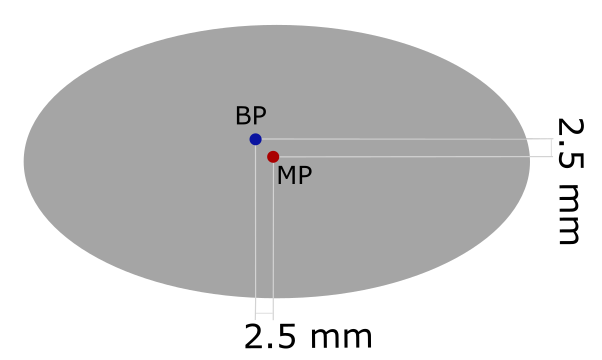
\includegraphics[width=8cm]{Images/validationcase/bluepoint/bluepointdiag.png}%
   \caption[Blue point - Diagram]{Blue point position diagram for the third validation case to evaluate the prediction of all force components.}%
   \label{fig:bluepointdiag}%
\end{figure}
To mimic the conditions of the experimental model II, the indentation depth was kept at $h_{VCIII}=\SI{4}{\milli \meter}$.
Based on the insights acquired from the deeper indentation validation case, it was considered 
prudent to maintain this depth to ensure that the selected material parameters would accurately 
represent the behavior of the specimen for this new indentation point.\\

In this use case, unlike the previous ones, the full computational model was required, as shown in Figure \ref{fig:bluepointcm}.
The symmetry boundary conditions used before were not applicable due to shifted indentation position.
With exception from these conditions the blue point model followed the process as computational model II, described 
in Section \ref{section:cmII}.

\begin{figure}
    \centering
    \begin{subfigure}[b]{0.5\textwidth}
    \centering
    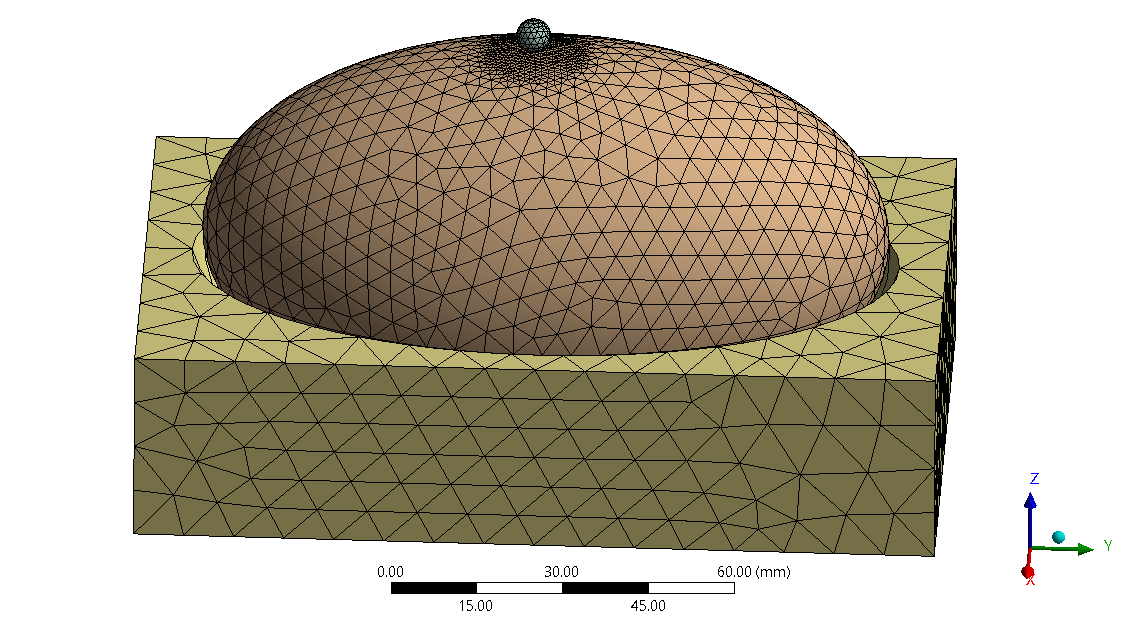
\includegraphics[width=\textwidth]{Images/validationcase/bluepoint/bluepointmesh.png}
    \caption{Full model geometry and mesh}
    \label{fig:bluepointgeoandmesh}
    \end{subfigure}
    \hfill
    \begin{subfigure}[b]{0.5\textwidth}
    \centering
    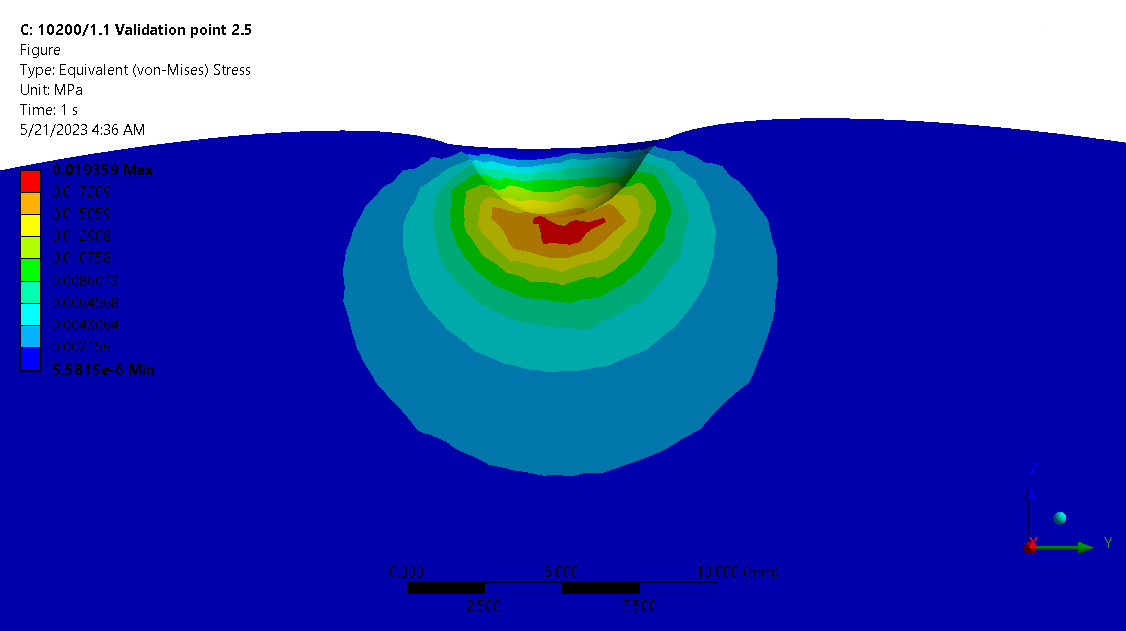
\includegraphics[width=\textwidth]{Images/validationcase/bluepoint/bluepointstress3.png}
    \caption{Von-Mises stress distribution}
    \label{fig:bluepointstress}
    \end{subfigure}
    \hspace{0.3cm}
    \caption[Blue point computational model]{Blue point computational model with use of the full geometry and stress distribution analysis.}
    \label{fig:bluepointcm}
\end{figure}

Furthermore, it was anticipated based on previous nearby point experiments that force components in 
x and y directions would become significant the further the indentation position was from the middle point (Subsection \ref{subsection:nearbypointresult}).
Hence, these components were included in the analysis alongside the z-direction force component.\\

The load displacement curves comparison for the middle and blue point revealed distinct behaviors.
For the middle point in Figure \ref{fig:mpforcecompvc}, the x-force component in the computational model was close to zero,
in comparison to the experimental data, which possessed a small but noticeable peak. 
Moreover, the simulation results for this force component appeared unstable.

On the contrary, the y-force component showed show a clear nonlinear trend in the computational model,
whereas the experimental curve showed minimal variation. The z-force component was previously analyzed 
and used to identify the material parameters, therefore has the closest match between the curves.

The total force curve exhibited a similar initial slope difference as showcased for the z-force component
However, after reaching a displacement of $u\approx\SI{1.2}{\milli \m}$, the simulation curve showed a increased slope,
diverging slightly from the experimental data.\\

The calculated NRMSE for all components and the total force reaction of the middle point test were listed in Table \ref{tab:forcecompnrmse}.
In the table was observed that the components for x and y showed high NRMSE values, but 
the z-component and the total force still lied below or slightly higher than the 
acceptable NRMSE limit of $\SI{0.1668}{}$.\\

\begin{table}[ht!]
    \centering
    \begin{tabular}{|>{\centering\arraybackslash}m{2cm}|>{\centering\arraybackslash}m{2.5cm}|>{\centering\arraybackslash}m{2cm}|>{\centering\arraybackslash}m{2cm}|}
    \hline
    Case & Force & NRMSE  \\
    \hline
    Middle Point & x-component y-component z-component Total & 1.1329 67.984 0.0534 0.1669 \\
    \hline
    Blue point & x-component y-component z-component Total & 0.1281 1.5615 0.0990 0.1015 \\
    \hline
    \end{tabular}
    \caption[Force components NRMSE]{Comparison of the NRMSE of all force components and total force reaction for the middle and blue point cases.}
	\label{tab:forcecompnrmse}
\end{table}

\begin{figure}[htbp]
    \centering
    %Fx
    \begin{subfigure}[b]{0.45\textwidth}
    \centering
    \begin{tikzpicture}[scale=0.78]
        \begin{axis}[
            xmax=4.2,xmin=0,
            ymin= -0.001,ymax=0.008,
            ytick={0,0.002,...,0.008},
            xlabel={Displacement $u [mm]$},
            ylabel={Force reaction $F [N]$},
            grid = major,
            legend pos= north west]
            \addplot+[smooth, no markers, thick] table [y=$Fx$, x=Def]{Table/results/bluepoint/midpoint/expmp.dat};
            \addplot+[smooth, no markers, thick] table [y=$Fx$, x=Def]{Table/results/bluepoint/midpoint/simmp.dat};
            \legend{EM II - MP, CM II - MP}
        \end{axis}
    \end{tikzpicture}
    \caption{X-force component}
    \end{subfigure}
    \hspace{0.3cm}
    \begin{subfigure}[b]{0.45\textwidth}
    \centering
    \begin{tikzpicture}[scale=0.78]
        \begin{axis}[
            xmax=4.2,xmin=0,
            ymin= 0,ymax=0.3,
            %ytick={0,0.1,0.2,...,0.6},
            xlabel={Displacement $u [mm]$},
            ylabel={Force reaction $F [N]$},
            grid = major,
            legend pos= north west]
            \addplot+[smooth, no markers, thick] table [y=$Fy$, x=Def]{Table/results/bluepoint/midpoint/expmp.dat};
            \addplot+[smooth, no markers, thick] table [y=$Fy$, x=Def]{Table/results/bluepoint/midpoint/simmp.dat};
            \legend{EM II - MP, CM II - MP}
        \end{axis}
    \end{tikzpicture}
    \caption{Y-force component}
    \end{subfigure}
    \vspace{0.5cm}
    \begin{subfigure}[b]{0.45\textwidth}
    \centering
    \begin{tikzpicture}[scale=0.78]
        \begin{axis}[
            xmax=4.2,xmin=0,
            ymin= 0,ymax=0.6,
            ytick={0,0.1,0.2,...,0.6},
            xlabel={Displacement $u [mm]$},
            ylabel={Force reaction $F [N]$},
            grid = major,
            legend pos= north west]
            \addplot+[smooth, no markers, thick] table [y=$Fz$, x=Def]{Table/results/bluepoint/midpoint/expmp.dat};
            \addplot+[smooth, no markers, thick] table [y=$Fz$, x=Def]{Table/results/bluepoint/midpoint/simmp.dat};
            \legend{EM II - MP, CM II - MP}
        \end{axis}
    \end{tikzpicture}
    \caption{Z-force component}
    \end{subfigure}  
    \hspace{0.3cm}
    \begin{subfigure}[b]{0.45\textwidth}
    \centering
    \begin{tikzpicture}[scale=0.78]
        \begin{axis}[
            xmax=4.2,xmin=0,
            ymin= 0,ymax=0.6,
            ytick={0,0.1,0.2,...,0.6},
            xlabel={Displacement $u [mm]$},
            ylabel={Force reaction $F [N]$},
            grid = major,
            legend pos= north west]
            \addplot+[smooth, no markers, thick] table [y=$Total$, x=Def]{Table/results/bluepoint/midpoint/expmp.dat};
            \addplot+[smooth, no markers, thick] table [y=$Total$, x=Def]{Table/results/bluepoint/midpoint/simmp.dat};
            \legend{EM II - MP, CM II - MP}
        \end{axis}
    \end{tikzpicture}
    \caption{Total force reaction}
    \end{subfigure}
    
    \caption[Middle point force components comparison]{Middle Point: Comparison and analysis of force components of the experimental data and the computational model.}
    \label{fig:mpforcecompvc}
\end{figure}
%blue point
The blue point case a greater alignment across for the x and y-components and the total force reaction, but
the NRMSE value for the z-component worsened from $\SI{0.0534}{}$ to $\SI{0.09}{}$ (Table \ref{tab:forcecompnrmse}).
In this validation case, the force components showed nonlinear trends in both the 
experimental and computational curves, with the simulation closely matching the
maximum forces obtained experimentally, with exception of the y-component, as 
illustrated in Figure \ref{fig:bpforcecompvc}.
This indicated that the identified parameters in set \SI{3}{} was suitable 
for the blue case as well, in addition to display more stable results for 
all load-displacements curves.\\

\begin{figure}[htbp]
    \centering
    %Fx
    \begin{subfigure}[b]{0.45\textwidth}
    \centering
    \begin{tikzpicture}[scale=0.78]
        \begin{axis}[
            xmax=4.2,xmin=0,
            ymin= 0,ymax=0.015,
            %ytick={0,0.002,...,0.008},
            xlabel={Displacement $u [mm]$},
            ylabel={Force reaction $F [N]$},
            grid = major,
            legend pos= north west]
            \addplot+[smooth, no markers, thick] table [y=$Fx$, x=Def]{Table/results/bluepoint/expbp.dat};
            \addplot+[smooth, no markers, thick] table [y=$Fx$, x=Def]{Table/results/bluepoint/simbp.dat};
            \legend{EM II - BP, CM II - BP}
        \end{axis}
    \end{tikzpicture}
    \caption{X-force component}
    \end{subfigure}
    \hspace{0.3cm}
    \begin{subfigure}[b]{0.45\textwidth}
    \centering
    \begin{tikzpicture}[scale=0.78]
        \begin{axis}[
            xmax=4.2,xmin=0,
            ymin= 0,ymax=0.05,
            %ytick={0,0.1,0.2,...,0.6},
            xlabel={Displacement $u [mm]$},
            ylabel={Force reaction $F [N]$},
            grid = major,
            legend pos= north west]
            \addplot+[smooth, no markers, thick] table [y=$Fy$, x=Def]{Table/results/bluepoint/expbp.dat};
            \addplot+[smooth, no markers, thick] table [y=$Fy$, x=Def]{Table/results/bluepoint/simbp.dat};
            \legend{EM II - BP, CM II - BP}
        \end{axis}
    \end{tikzpicture}
    \caption{Y-force component}
    \end{subfigure}
    \vspace{0.5cm}
    \begin{subfigure}[b]{0.45\textwidth}
    \centering
    \begin{tikzpicture}[scale=0.78]
        \begin{axis}[
            xmax=4.2,xmin=0,
            ymin= 0,ymax=0.6,
            ytick={0,0.1,0.2,...,0.6},
            xlabel={Displacement $u [mm]$},
            ylabel={Force reaction $F [N]$},
            grid = major,
            legend pos= north west]
            \addplot+[smooth, no markers, thick] table [y=$Fz$, x=Def]{Table/results/bluepoint/expbp.dat};
            \addplot+[smooth, no markers, thick] table [y=$Fz$, x=Def]{Table/results/bluepoint/simbp.dat};
            \legend{EM II - BP, CM II - BP}
        \end{axis}
    \end{tikzpicture}
    \caption{Z-force component}
    \end{subfigure}  
    \hspace{0.3cm}
    \begin{subfigure}[b]{0.45\textwidth}
    \centering
    \begin{tikzpicture}[scale=0.78]
        \begin{axis}[
            xmax=4.2,xmin=0,
            ymin= 0,ymax=0.6,
            ytick={0,0.1,0.2,...,0.6},
            xlabel={Displacement $u [mm]$},
            ylabel={Force reaction $F [N]$},
            grid = major,
            legend pos= north west]
            \addplot+[smooth, no markers, thick] table [y=$Total$, x=Def]{Table/results/bluepoint/expbp.dat};
            \addplot+[smooth, no markers, thick] table [y=$Total$, x=Def]{Table/results/bluepoint/simbp.dat};
            \legend{EM II - BP, CM II - BP}
        \end{axis}
    \end{tikzpicture}
    \caption{Total force reaction}
    \end{subfigure}
    
    \caption[Blue point force components comparison]{Blue Point: Comparison and analysis of force components of the experimental data and the computational model.}
    \label{fig:bpforcecompvc}
\end{figure}

In conclusion, the third validation case reinforced the validity of set number
\SI{3}{} as the chosen parameter set for this study. This set 
demonstrated an acceptable level of agreement for all cases with an equal 
indentation depth. Moreover, this validation supported that this material model 
can model the behavior of the polyurethane specimen under indentation, particularly
when considering different locations on the specimen's surface and all 
force components into the analysis.
%--------------------------------------------------------------------------------------------------
\section{Framework Proposal}
With this study a framework for the identification of soft material's parameters, focusing on the 
simplest possible material model was proposed. This framework, illustrated in Figure \ref{fig:flowchart}, 
was based on an iFEM approach and provided a robust and systematic procedure that aligns experimental 
load-displacement data with computational models.\\

This process began with defining the use case and proceeded with the inclusion of two primary paths
running in parallel; the design of the experimental model or comparator, and the computational or FE model.

On the experimental design side, the physical indentation experiments were design and performed (Experimental 
Model I and II). During these experiments, the mechanical behavior of the material was observed and analyzed.
This analysis played a crucial role in establishing the main assumptions for the material model. Furthermore, 
load-displacement data was captured, which served as the benchmark 
against which the computational model was verified.\\

On the computational model design side, the corresponding simulation was constructed to meet the experimental 
conditions. Here, the simplest material law was selected and initial parameters were set, allowing for the simulation of 
the indentation process and generation of load-displacement data.\\

The simulation load-displacement data was then compared with the measured data from the experiments.
An important inquiry at this stage was wether the selected material law adequately capture the mechanical 
behavior of the material. If the answer was no, the material law was adjusted to the next level, and the 
simulation was rerun. This loop continued until a satisfactory agreement was found.\\

Once the simulation captured the mechanical behavior, the material parameters' or design parameters were inputted into a 
response surface optimization process. Here, the definition of an adequate range, played an important role 
in the obtained candidate sets.\\ 

The next step, involved running the simulations for the different candidate points or material parameter sets,
an calculating their pre-established error metric. This error metric, such as NRMSE, was used to determine 
wether these simulations met ir surpassed the established error threshold. If the simulation did not meet the threshold, 
the process was repeated with new sets of candidate material sets.\\

Finally, once a parameter set met the error threshold, it was identified as the optimal material parameter set.
This was an iterative and comprehensive process that ensured that the identified material 
parameters were not only theoretically robust but also practically validated.
This proposed framework is a tool for the identification of material parameters to describe a complex material behavior,
representing a balance between simplicity and accuracy. 


\begin{figure}%   
    \begin{center}
    \begin{tikzpicture}[node distance = 0.5cm, auto, thick]
        \tikzstyle{decision} = [diamond, draw, text width=4em, text badly centered, node distance=0.5cm, inner sep=0pt, font=\small]
        \tikzstyle{block} = [rectangle, draw, text width=6.5em, text centered, rounded corners, minimum height=3.5em, font=\small]
        \tikzstyle{line} = [draw, -latex']
    
        \node [block] (start) {Definition of Use Case};
    
        \node [block, below right =of start,xshift=0.75cm] (process1) {Experimental design};
        \node [block, below =of process1,yshift=-3.8cm] (process2) {Measured load-displacement};
    
        \node [block, below left=of start,xshift=-0.75cm] (process5) {FE Model design};
        \node [block, below =of process5] (process3) {Selection of material law};
        \node [block, below =of process3] (process4) {Initial parameter set};
        
        \node [block, below =of process4] (process6) {Simulated load-displacement};
    
        \node [block, right =of process6, xshift=0.7cm] (process7) {Comparison of data};
        \node [decision, below =of process7] (decision1) {Capture mechanical behavior?};
    
        \node [block, below =of decision1] (success1) {Input material parameters' range in RSO};
    
        \node [block, below =of success1] (process8) {Simulate candidate points};
    
        \node [decision, below =of process8] (decision2) {Error metric threshold?};
        \node [block, below =of decision2] (success2) {Optimal material parameter set};
    
        \path [line] (start) -- (process1);
        \path [line] (start) -- (process5);
    
        \path [line] (process1) -- (process2);
        \path [line] (process2) -- (process7);
    
        \path [line] (process5) -- (process3);
        \path [line] (process3) -- (process4);
        \path [line] (process4) -- (process6);
        \path [line] (process6) -- (process7);
    
        \path [line] (process7) -- (decision1);
        %\path [line] (decision1) -| node [near start] {no} ($(process3.west)+(-1,0)$);
        %\path [line] ($(process3.west)+(-1,0)$) -- (process3);
        \path [line] (decision1) -|  node [near start] {no} ($(process3.west)+(-1,0)$) -- (process3);
        \path [line] (decision1) -- node {yes} (success1);
    
        \path [line] (success1) -- (process8);
        \path [line] (process8) -- (decision2);
        
        %\path [line] (decision2) -| node [near start] {no} ($(success1.west)+(-1,0)$);
        %\path [line] ($(success1.west)+(-1,0)$) -- (success1);
        \path [line] (decision2) -|  node [near start] {no} ($(success1.west)+(-1,0)$) -- (success1);

        \path [line] (decision2) -- node {yes} (success2);
    
    \end{tikzpicture}
    \end{center}
    \caption[Framework proposal]{Flowchart of the identification of soft material parameters based on an iFEM approach conducted in this study.}%
    \label{fig:flowchart}%
 \end{figure}
     

%------------------------------------------------------------------------------------------------
\section{Limitations and Implications of the Results}
The findings from this study offered valuable insights for the identification of soft material 
parameters. However, it is essential to acknowledge the limitations of the proposed framework and 
the obtained results, as well as their implications on its applicability.\\

One notable limitation arose from the indentation depth used for the identification process. 
As the indentation depth increased, the accuracy of the material model decreased significantly.
Additionally, maintaining the stability of the computational model became increasingly 
difficult with a larger indentation due to element large deformation issues. This
issue was addressed using the nonlinear adaptive meshing option, although it added 
another layer of complexity to the FE modeling process.\\

The proposed method demonstrated positive performance for simple testing scenarios, such 
as vertical indentation and small deformations. As the complexity of the use case increased,
the challenge of finding a simple material model capable of accurately replicating the material 
behavior became more pronounced. 

An additional limitation was discovered in the analysis of the deformation profile.
It was observed that the Neo-Hookean model could match the experimental deformation
profile at a single point but failed to reproduce the entire measured deformation shape.
This indicated that a refinement in the experimental procedure, or the selection of a 
different material model may be necessary to improve the results.\\

Assumptions made in this study also contributed to certain limitations. The assumed symmetrical
deformation might not be applicable to all materials, thereby constraining the framework's
utility. Furthermore, the choice of the middle point for the experimental model was based on
simplicity and avoid external factor that could influence in the selection of the material 
model. Nonetheless, this point was not optimal to accurately capturing all force reaction 
components.\\

The material parameters' range used in the RSO process affected the obtained candidate points, 
demonstrating a sensitivity to defined ranges. Noticeably, the best material parameter set 
found originated from the approximated polynomial global minimum obtained from the MATLAB code, 
suggesting the potential for further optimization of the range inputted in the RSO process. 
Despite this, set \SI{1}{}, the best candidate from the RSO process, demonstrated comparable 
results to the MATLAB set, reinforcing the validity of the proposed methodology.\\

Lastly, this study highlighted the significance
of balancing simplicity and accuracy in material parameter identification process for ultra-soft polyurethane. 
While the proposed methodology effectively handled simpler cases, the results indicated
the need for a more sophisticated approach when dealing with complex deformation scenarios.
These findings can provide useful insights and a valuable foundation for further refinement and 
improvement of parameter identification methodologies.







%\subsection{First Experimental model}
%The chosen experimental technique for the inverse identification for this project was indentation. 
%The test specimen used for this experiment was a ultra-soft polyurethane resin. 
%As shown in Fig.. the specimen possesses a ellipsoidal form with 
%with a minor radius \(r_1\) = 35 mm and a major radius \(r_2\) = 60 mm. This was positioned
% on a fixed platform that suited the ellipsoidal geometry of the 
% specimen to constrain its movement. 
% The specimen was tested in a indentation test configuration with a tensile/compression machine.
% To achieve this congiguration a pin with a rounded head made of structural steel, 
% with a radius of \(r_3\) = 3 mm was attached 
% to the holding grips followed by a force load cell. 
%The result of indentation test was a load-displacement points. The approximated 
%polynomial curve was used as a reference for the material modeling.

%test specimen is loaded at a quasi-static rate

% The measured force reation \(F_1\) data showed a very small number, so the 
% first 50 N load cell displayed a lot of noise in the measurements. 
% Therefore, the load cell was change to 10N to reduce this interference. 
%The 10 N load cell displayed the force-displacement curve of the indenter and the specimen
% in a finer way. Furthermore, in order to get the measurement of the load and 
% unloading process of
% the indentation a displacement sensor was attached to the tensile machine.

% The indentation depth \(h_1\) selected for the first model was 3,8 mm on the middle of the 
% top surface of the specimen. This indentation depth surpasses the pin radius \(r_3\) and 
% was chose arbitriarily to analyze the behavior of the material on the defined position.
 %reference?


%\begin{figure}[th]
%    \centering
%    \begin{tikzpicture}
%        %\pgfplotsset{%legend outside the plot
%        %every axis legend/.append style={ at={(1.05,0.95)}, anchor=north west,legend columns = 1}}
%        \begin{axis}[
%            %axis lines=middle,
%            %x label style={at={(axis description cs:0.5,-0.1)},anchor=north},
%            %y label style={at={(axis description cs:-0.1,.5)},rotate=90,anchor=south},
%            xlabel={Displacement $u [mm]$},
%            ylabel={Force reaction in Z-Axis $F_z [N]$},
%            legend pos= north west]
%            
%            \addplot+[smooth, mark size = 1pt] table [y=$Force$, x=Def]{Table/data1.dat};
%            %\addplot+[smooth] table [y=Force, x=$Def$]{Table/data2.dat};
%            \legend{Experimental data}%,$l_2$}
%        \end{axis}
%    \end{tikzpicture}
%    \caption[Expdata]{Experimental Load-displacement curve.}
%    \label{fig:testgraph2}
%\end{figure}

%\subsection{Second Experimental model}
%The second experimental model was developed by Yokohama National University. Similar to 
%the first experimental model the test specimen and the platform were it lies, has the 
%same dimensions, minor radius $r_1 = \SI{35}{\milli \m}$ and a major radius \(r_2\) of 60 mm. The
%test specimen is also made from the same material, ultra-soft polyurethane resin.
%
%The indenter on the other hand, is a sphere made of ruby, the sphere radius is also 
%equal to the radius of the pin \(r_s\) 3 mm and attached to it, is the force load cell.
%
%A laser is used to measure the displacement which results in a load-displacement curve.
%With this model it is possible to not only determine the toal force reaction, but also
%it's components \(F_x\),  \(F_y\) and \(F_z\). Furthermore, with the laser it is also
%possible to observe the deformation not only in one point but around the whole area. 
%This allows as to analyze the deformation of the whole structure.
%
%The indentation speed selcted was % ask for which speeed
%and with an indentation depth of \(h_s\) is 4 mm. With this experiment, 4 key points on 
%the sepcimen's surface were chosen: First, in the middle and three other points, one to right, 
%one down, and one diagonal to middle, forming a square with a distance between points 
%of \(d_s\) 20 mm. %add figure with points

%----------------------------------------------------------------------------------
%\section{Material model framework assumptions}
%
%The first point to be analyzed, which is used to build a material model is point No. 1,
%in the middle of the surface. The advantages from this case, is the less influence of
%external factors. For this case it is vaiable to assumed, that shear stresses can be 
%neglected and offers a simple model to focus on the material definition.
%
%For this project, there is a focus on the limitation of each material model, 
%departing from an ideal scenario. From this point on the material will be build 
%accordingly and for each model the influence of the material parameters is going
%to be assessed.

%Por revisar!!!
%----------------------------------------------------------------------------------
%\section{Material model}

%n an ideal and first scenario, this material can be assumed as linear, isotropic, 
%lastic and nearly imcompressible. For this case, there are two main variables, the Young's
%odulus \(E\), and the Poisson's ratio $\nu$.

%comentario sobre la influencia del bulk modulus y poissons ratio
%From the parametric analysis, it is possible to see that the bulk 
%modulus of this material does not possess a big impact in the FE 
%simulation results. This conclusion combined with the results 
%from the Poisson ratio in the first material model coincide with the 
%statements from Bergström, where it is no vital to know these parameters 
%to obtain accurate FE computational models, as these have limited
%influence on the mechanical response. \cite{Bergström2015} %pag64Bergströom

%---------------------------------------------------------------------------------

%Additionally, it was observed that in soft materials it is easier to capture 
%some parameters with a larger indentation. Some references also observe that with
%indentation depth lower than indenter radius has a lot of noise and do not describe
%th results accurately. %reference?